 \documentclass[12pt,a4paper]{article}
\usepackage[utf8]{inputenc}
\usepackage{amsmath}
\usepackage{amsfonts}
\usepackage{amssymb}
\usepackage{gensymb}
\usepackage{graphicx} %package to manage images
\usepackage{siunitx}
\graphicspath{ {./images/} }
\usepackage[show]{chato-notes}
\newcommand{\ceg}[1]{\mynote[author=EG]{#1}}
\newcommand{\cvt}[1]{\reply[author=VT]{#1}}
\author{Viet Ta}
\title{Mining redescriptions from Boolean data with a hierarchy}
\begin{document}
\maketitle

With the enormous amount of data we produce nowadays, data mining is becoming more and more prevalent. Consequently, the goal with modern data mining methods is not only to discover information from crude data, but also to condense that information down to concise descriptions and insights. One such method is redescription mining~\cite{ramakrishnan_turning_2004}. In a nutshell, it aims to find different ways to describe the same things.

Redescription mining can be applied in many fields, including for instance biology, ecology, social and political sciences~\cite{galbrun2018redescription}.
A classic example of redescription mining application is in finding bio-climatic niches, or, in other words, relate the habitat of particular species or groups of species, to the local climatic conditions.
In this example, we want to describe geographic regions in terms of the fauna that inhabits them, on one hand, and in terms of the values of some climatic variables, on the other hand. In particular, the aim of redescription mining is to extract such pairs of descriptions automatically from a given dataset.
As a specific example, the method might return a redescription that states that areas where the maximum temperature in March is between \SI{-24.4}{\degreeCelsius{}} and \SI{4.3}{\degreeCelsius{}} are roughly the same as area inhabited by lynxes (see Figure~\ref{fig:niche}).
In this application, the aim is to help ecologists understand the impact of climate on the distribution of species.

\begin{figure}[bt]
 \centering
 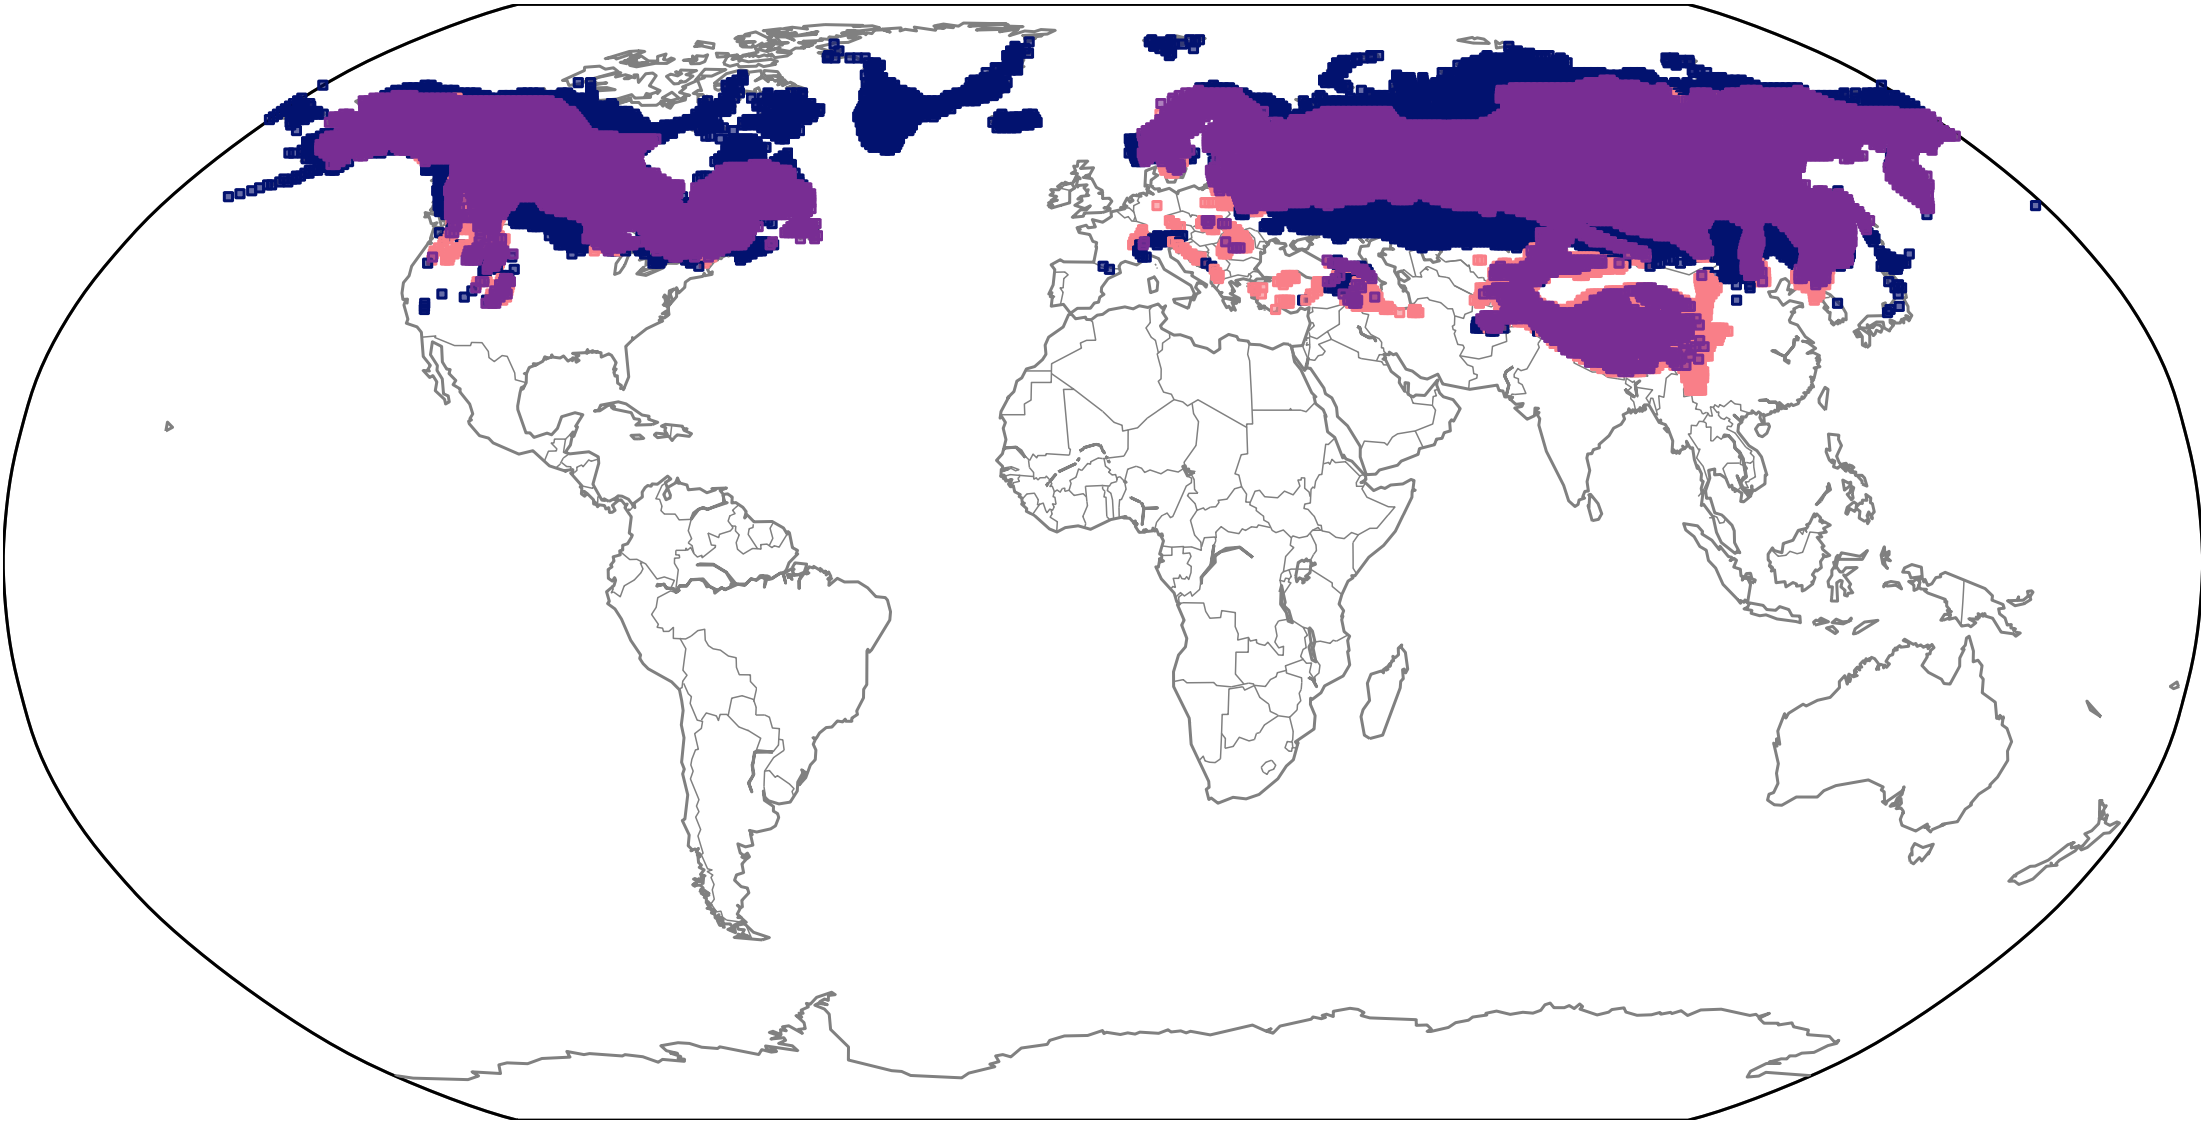
\includegraphics[width=10cm]{niche-finding}
 \caption{An example redescription plotted on a map, showing the areas inhabited by lynxes (light red and medium purple) and the areas where the maximum March temperature is between \SI{-24.4}{\degreeCelsius{}} and \SI{3.4}{\degreeCelsius{}} (dark blue and medium purple) \cite{galbrun2018redescription}}
 \label{fig:niche}
\end{figure}


Here we follow the formalism of \cite{Galbrun-Methods}.
The input of redescription mining is a dataset that consists of a set of \emph{entities} described by a collection of \emph{attributes}.
The attributes are partitioned into disjoint \emph{views} that correspond to logical groups of attributes. Each view can be thought of as a data table, where the columns represent the attributes, and the rows represent the entities, which map across the different tables.
In the bioclimatic-niche finding example above, the entities are geographic locations and the views correspond to species occurrences and climate, respectively.
That is, one view contains attributes that each record the presence or absence of a specific species in each location, whereas the other view contains attributes that each record the value taken by a specific climatic variable in each location.
This can be represented as a pair of tables, as shown in Table~\ref{tab:mammals-and-climate}.

\begin{table}[tb]
\resizebox{\textwidth}{!}{%
\begin{tabular}{|l|l|l|l|l|l|l|l|l|l|l|l|}
\cline{1-6} \cline{8-12}
\multicolumn{6}{|c|}{Species occurrences} &  & \multicolumn{5}{c|}{Climate}                                  \\ \cline{1-6} \cline{8-12} 
Location ID   & mountain hare & \dots & Canada lynx   & Eurasian lynx  & \dots  &  & Location ID & \dots & max.\ March T.\ & avg.\ May P.\ & \dots \\ \cline{1-6} \cline{8-12} 
\dots  & \dots & \dots & \dots   & \dots  & \dots &  & \dots  & \dots & \dots & \dots & \dots \\ \cline{1-6} \cline{8-12} 
4652 & True  & \dots & True  & False & \dots &  & 4652 & \dots & 2   & 10  & \dots \\ \cline{1-6} \cline{8-12} 
4653 & True  & \dots & False & True & \dots &  & 4653 & \dots & 3   & 40  & \dots \\ \cline{1-6} \cline{8-12} 
\dots. & \dots & \dots & \dots   & \dots  & \dots &  & \dots. & \dots & \dots & \dots & \dots \\ \cline{1-6} \cline{8-12} 
\end{tabular}%
}
\caption{An example dataset, represented as a pair of data tables with mapped rows. The left-hand side table records occurrences of various species, while the right-hand side table records the values of various bio-climatic variables such as temperature (T, in \si{\degreeCelsius{}}) and precipitation (P, in \si{\milli\meter}).}
\label{tab:mammals-and-climate}
\end{table}

Then, a description, or query, is a logical formula over attributes.
The query can be evaluated for each entity, and returns a Boolean value that indicates whether the entity satisfies the query conditions.
The support of a query is the set of entities that satisfy the query.
A redescription is then a pair of queries, respectively over attributes from distinct views, having sufficiently similar supports \cite{galbrun2018redescription}.
In the bioclimatic-niche finding example above, a redescription consists of a query over species occurrences and over climatic variables, respectively, that are satisfied in roughly the same locations.

Different redescription mining algorithms have been proposed, that use different strategies, handle different types of attributes and allow different types of constraints on the queries \cite{galbrun2018redescription}.
Here, we focus on datasets containing Boolean attributes arranged into a hierarchy.
Boolean attributes can be viewed as special case of categorical attributes with only two possible values, \texttt{True} and \texttt{False}.
A hierarchy is a logical structure that organises the attributes into different levels, which can be represented as a pyramid or a tree.

% what's special about Boolean data algorithms?
The problem of Boolean attributes with a hierarchy is an interesting scenario where an additional dimension is introduced into the data structure. 

The hierarchical information can be stored separately or embedded into the attributes names, e.g.\ through prefixes. 
In fact, in the bio-climatic niche finding example, hierarchical information is available about the attributes of the species occurrence table. Indeed, in biology all species are classified in a taxonomic hierarchy and given a two-part name, where the first part represents the genus to which the species belongs. The Canada lynx and Eurasian lynx, a.k.a.\ \textit{Lynx canadensis} and \textit{Lynx lynx}, respectively, both belong to the same wild cat genus \textit{Lynx}. However, this information is not currently taken into account when mining redescriptions. Higher levels of the taxonomic hierarchy could also be incorporated.

Hierarchical information could be used to impose refined constraints on the queries, or to design optimized mining algorithms. Depending on the application, it could be of interest, for instance, to forbid siblings in the hierarchy to appear together in a query.
On the other hand, the hierarchical information can be exploited to prune candidates more efficiently during the mining process. For instance, if we find out that a parent attribute has a low support, we might automatically prune its children from the search space.
\bibliographystyle{apalike}
\bibliography{references}
\end{document}